\section{Demonstrator Prototype}
\label{sec:prototype}

\subsection{The Prototype}
The prototype we built as our project was a microservice based Java EE application for keeping track of available offices at Western Norway University of Applied Sciences. The application architecture was inspired by the model-view-controller architectural pattern, but the prototype is currently lacking the view component. We implemented three independent microservices (models) which, together with a controller/gateway (controller), constitute our prototype. 

\subsubsection{Functionality}
Due to limited time, we were not able to implement all of the components we decided on initially. We decided on implementing the model and controller components so that we would have a working backend. For testing, we decided to use postman to simulate client requests that eventually will be generated by user interaction, and sent from a front end service.  \\
\newline
The prototype includes the following functionality:
\begin{itemize}
    \item Create user
    \item Mark an office as available
    \item Update office information
    \item Create new offices
    \item Book an available office
    \item Get a list of available offices, and the period they are available for
    \item Authenticate a user requesting a resource
    \item Generate session tokens
\end{itemize}

\subsubsection{Project Architecture}
Our system design, as seen in figure x (replace x with fig. num), consists of three services and a gateway/controller. The controller serves as an entry point for user requests. Its main purpose is to forward requests to the appropriate service and return the response to the client. The controller decouples the services from the clients so that the services can be updated or refactored without having to update all clients. We also built three independent and loosely coupled services implementing the business logic, each with their own database so that they can persist their own data. The purpose of the services is to process client requests forwarded by the controller and return a response. The controller communicates with the services through REST APIs, where data is sent as headers.

\begin{figure}[ht]
  \centering
  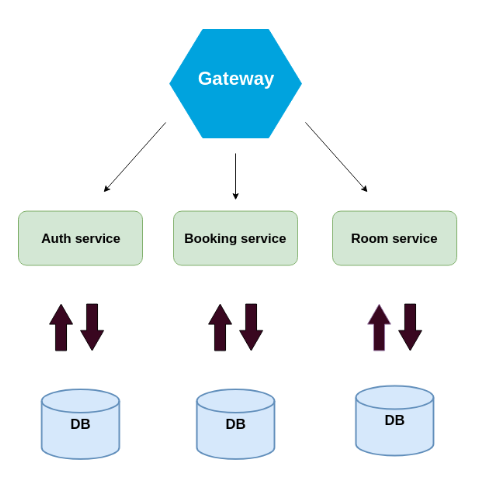
\includegraphics[scale=0.8]{figs/projectArchitecture.png}
  \caption{Project Architecture}
  \label{fig:projectarch}
\end{figure}
\newpage
\subsubsection{The Development Process}
One benefit of the architecture we had decided on, is that the services could be independently developed and tested since the services don’t depend on each other. The services were “bound” together by the controller, resulting in a pretty complex system compared to if we would have implemented the same system as a monolith. A monolithic architecture would have been easier to implement, but at the cost of independent components. Our motivation for this project was to research microservice technologies, so that is what we went with. \\
\newline

\noindent Since Thorntail is a framework for developing enterprise Java applications, we had the opportunity to use some of the same frameworks and APIs we used when developing the auction application. We decided to continue using the framework JAX-RS, to set up our REST communication, and the API JPA, for object-relational mapping. We also decided that each microservice should persist their own data in an embedded H2 relational database. 


\subsubsection{Getting Started}
Thorntail provides a project generator which generates a maven project for you based on the dependencies you choose (fig. x) at: \hyperref[https://thorntail.io/generator/]{https://thorntail.io/generator/} \\

\noindent You have the opportunity to add only the dependencies you need or none at all. The maven plugin also auto-detect dependencies added during the development process, so you don’t need to know exactly what dependencies you are going to need when starting a project.

\begin{figure}[ht]
  \centering
  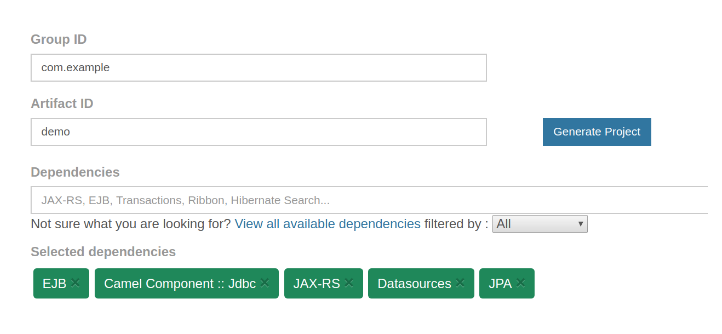
\includegraphics[scale=0.7]{figs/thorntailgenerator.png}
  \caption{Thorntail Generator with selected dependencies}
  \label{fig:thorntailgenerator}
\end{figure}

\subsubsection{Database}
In our application we needed each microservice to store the application data, and the authentication service to keep track of session tokens. As for how to store the data, we went with embedded H2 databases. To set up a H2 database, all we had to do was to configure the datasource in the project-defaults.yml file as seen in figure x.\\

\begin{figure}[ht]
  \centering
  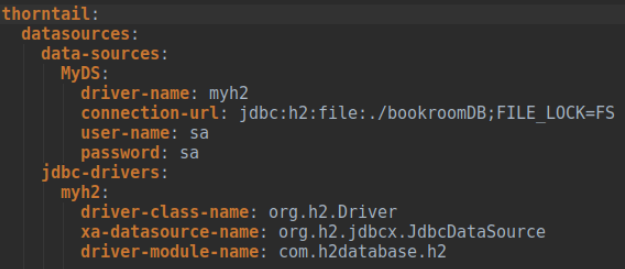
\includegraphics[scale=0.9]{figs/databaseconfig.png}
  \caption{Database Configuration}
  \label{fig:databaseconfig}
\end{figure}
\newpage
\noindent A new, empty database will be created if the database specified in the URL doesn’t exist. The mapping between the databases and the application objects is defined by persistence metadata. In our project, the JPA metadata is defined by annotations and used to perform different database operations. In this way, we were able to work with the objects of our system, instead of writing SQL statements. The javax.persistence.Entity  (beautify in latex) annotation makes an entity class, and \textbf{javax.persistence.Column} defines the columns of the tables. JPA will create tables in the database corresponding to the persistence metadata. The \textbf{javax.persistence.EntityManager} provides four basic operations of persistent storage that we made use of in our project:

\begin{itemize}
    \item Persist, to add new objects to the database
    \item Find, to find and return an object/objects
    \item Merge (edit), to update an object
    \item Remove, to delete an object
\end{itemize}

\noindent The persistence.xml describes the persistence unit, and the persistence unit configures the EntityManager. The EntityManager instance manages the entities by using the PersistenceContext, and it can be injected via the \textbf{@PersistenceContext} annotation, as shown in figure x. Entity instances and lifecycles are managed within the scope defined by the PersistenceContext. The EntityManager serves as a reference to the PersistenceContext associated with a transaction. The PersistenceContext is pretty much a cache which contains a set of persistent entities. When a transaction is committed, the persistent objects are detached from the PersistenceContext, and it is flushed and cleared.\\

\begin{figure}[ht]
  \centering
  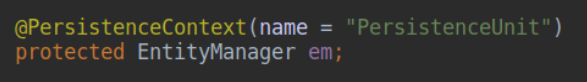
\includegraphics[scale=0.9]{figs/persistencecontext.png}
  \caption{PersistanceContext}
  \label{fig:databaseconfig}
\end{figure}

\newpage

\subsubsection{Communication}
The services in our prototype communicate with the controller using rest APIs. Each microservice has its own rest API with endpoints triggered by incoming requests from the controller. Figure x shows an example endpoint from the authentication service that is triggered when a session token needs to be verified. This method returns a boolean value to the controller, letting it know whether the token is valid or not. \\

\begin{figure}[ht]
  \centering
  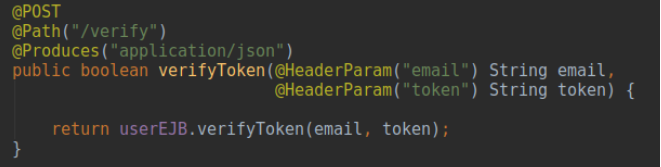
\includegraphics[scale=0.9]{figs/verifyendpoint.png}
  \caption{Verify Endpoint}
  \label{fig:databaseconfig}
\end{figure}

\noindent Triggering this endpoint will call the backend logic for verifying a user’s token, shown in figure x. The method fetches the user with given email from the database or throws an exception if the user doesn’t exist. If the user has an active session, i.e. \textit{user.getAuthToken()} does not return null, the stored session token it is matched against the token that came with the request. If they are identical, the user will be verified, otherwise, the user will not be verified.  

\begin{figure}[ht]
  \centering
  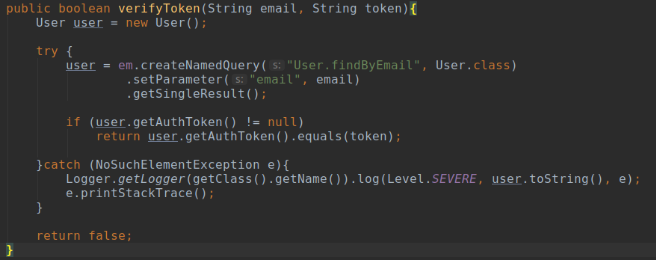
\includegraphics[scale=0.9]{figs/verifytoken.png}
  \caption{Verify Token}
  \label{fig:verifytoken}
\end{figure}
\newpage
\noindent The endpoints in the controller are triggered by incoming user requests. When a client requests a resource, the controller opens an HTTP connection to the appropriate resource’s URL, sends a POST request with the headers from the incoming request, and fetches the answer from the service. Figure x shows a method for sending requests and fetching a response from the controller, taking an URL and headers as parameters. The fetch will either return a response or null if there was an error, in which case it will Log a warning with the response code. \\

\begin{figure}[ht]
  \centering
  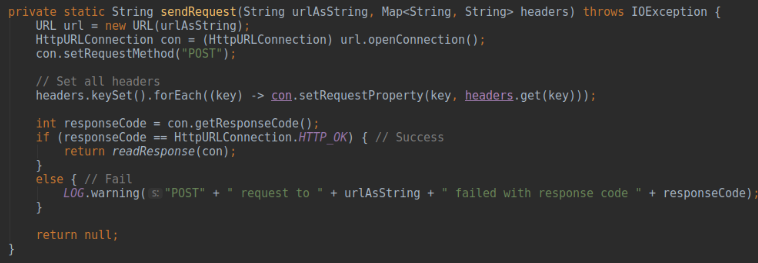
\includegraphics[scale=0.75]{figs/sendrequest.png}
  \caption{Send Request}
  \label{fig:databaseconfig}
\end{figure}

\noindent An example of session token verification is shown in figure y. The controller sets the headers to match the corresponding headers of the incoming client request, i.e. email address and session token and sends it using the method in figure x. The verify method will return the result from the sendRequest method. This means that triggering the verify endpoint will result in either true (valid), false (not valid), or a connection error.\\

\begin{figure}[ht]
  \centering
  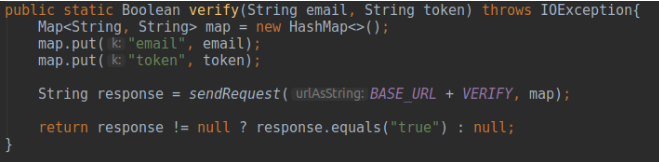
\includegraphics[scale=0.75]{figs/verify.png}
  \caption{Verify}
  \label{fig:databaseconfig}
\end{figure}

\noindent Throughout the whole system, requests are sent and processed in a similar manner as explained above. The only difference between requests is features specific to each request, such as the URL of the resource endpoint, and which headers to send with the request. Responses are also requested specifically. A successful log-in, for instance, will return a session token, while the session token verification returns a boolean. As mentioned earlier, the controller controls the flow of requests and forwards them to the appropriate backend service, where the requests are processed, and a proper response returned to the controller. 

%\lstinputlisting[language=java]{code/BoksVolum.java}
